\documentclass[]{article}

\usepackage{fullpage}
\usepackage{graphicx}
\usepackage{amsmath}
\usepackage{amsfonts}
\usepackage[colorlinks=true, allcolors=blue]{hyperref}

%Use Charter font
\renewcommand{\familydefault}{bch}

%opening
\title{Bullet-Fluids Reference (draft version)}
\author{}
\date{02 January 2014}

\begin{document}

\maketitle

\begin{abstract}
	Originally based on Fluids v.2 \cite{RH:2008}, the Bullet-Fluids library is a Zlib licensed extension to the Bullet
	Physics engine \cite{EC:2012} that is targeted at interactive or real-time simulation of fluids using the meshless 
	particle method known as SPH.\\
	
	The library is being developed as a draft for the production version, which is targeted at Bullet 3.x.\\
	
	This document provides an introduction to the Bullet-Fluids library, and also includes some explanation of 
	parameters and other details.
\end{abstract}

\tableofcontents

\pagebreak
\section{Introduction to Bullet-Fluids}
	\label{s_bulletFluidsIntro}
	
	\subsection{Important notes (please read this section before using the library)}
		\subsubsection{Simulation Scale}
			\label{s_simulationScale}
			The fluid simulation defines two scales, \textit{world scale} and \textit{fluid simulation scale} 
			(hereafter, \textit{simulation scale}).
			\begin{itemize}
				\item \textit{simulation scale} is the scale at which the SPH density and forces are calculated.
				\item \textit{world scale} is the scale at which rendering, the rigid body simulation and all other functions take place.
			\end{itemize}
			
			In general, the world scale is much larger than the simulation scale. Multiplying a value by the simulation 
			scale can be seen as scaling down the value from world or rigid body units to fluid units, while dividing a 
			value by the simulation scale is equivalent to scaling up the value from the fluid simulation scale to world units.
			
			\[ \mathbf{simulation\_scale\_length = world\_scale\_length * simulation\_scale} \]
			\[ \mathbf{world\_scale\_length = simulation\_scale\_length / simulation\_scale} \]
			
			To give a concrete example, the default simulation scale is 0.004.\\
			This means that a length of 1 metre at world scale is shrunk to 0.004 metres at simulation scale.\\
			Alternatively, a length of 1 metre at simulation scale is expanded to 250 metres at world scale.\\
			In either case, the ratio of world scale to simulation scale is (1 / simulation\_scale), or 1 : 250 by default.\\
			
			When changing the size of the particles, it is recommended to change m\_simulationScale and parameters 
			marked [world scale]. Reducing the simulation scale will make particles larger, and increasing it will 
			make the particles smaller. For example, doubling the default simulation scale of 0.004 will halve the 
			size of the particles. (default: 1 / 0.004 = 250; halved: 1 / 0.008 = 125).\\
			
			Although in theory it should only be necessary to change the simulation scale to resize the fluid, in practice
			floating point rounding can cause the fluid to behave differently when the simulation scale is changed. (Even if
			there is no difference mathematically.) However, this should not matter unless the simulation scale is changed by
			a factor of 100-1000x or greater.\\
			
			The motivation for including the simulation scale parameter is to provide a easy way to change the scale of
			the fluid without affecting its behavior. The Navier-Stokes equations are sensitive to scale, and so the SPH
			approximation of their terms is also scale sensitive.\\
			
			Additionally, SPH is highly sensitive to the parameters used; if a single parameter is even slightly incorrect, 
			it can cause the entire simulation to explode. Abstracting the size of the fluid using a `simulation scale' term
			allows us to shrink or expand the fluid without spending excessive effort on tuning the parameters. Were the 
			simulation scale not implemented, it would be a difficult task to get all parameters correct on the first try. 
			Using two scales allows us to make slight modifications from a working set of parameters to get the desired 
			behavior.\\
			
			Some more details on the simulation scale are provided at the Fluids v.2 website \cite{RH:2008}.
			
		\subsubsection{Changing Particle Indicies}
			The particle data is resorted every frame. For instance, the particle at index 0 could in the next frame be
			at index 3, or some other location. This means that the index of each particle cannot be used to track it. 
			However, each particle has a user pointer that can be used to associate a unique id or struct with it. The 
			per-particle user pointer can be accessed through btFluidSph::getParticleUserPointer() and 
			btFluidSph::setParticleUserPointer(). This user pointer is set to 0 when the particle is created, and is 
			sorted along with the particle data every frame. It is not modified otherwise.\\
			
			Alternatively, the fluid's grid(accessible through btFluidSph::getGrid()) stores the previous indices
			of the particles. It can be accessed with btFluidSortingGrid::getValueIndexPairs().\\
			
			The main reason for rearranging the particle data is performance; sorting the particles increases the cache 
			hit rate.
		
		\subsubsection{Explosions}
			A common issue that may be encountered when implementing a SPH fluid simulation is the `explosion', where 
			the particles cease to behave as a fluid and begin to fly around everywhere.\\
			
			This issue is usually caused by applying very high forces to the fluid particles. The source of such forces 
			is many; it could occur if any of the following is set too high: time step, stiffness, gravity, viscosity 
			or other user applied forces. The most sensitive of these parameters are the time step and stiffness.
	
	\subsection{Class Heirarchy}
		There are 2 main classes, and those 2 classes contain 5 important subclasses.
	
		\subsubsection{btFluidRigidDynamicsWorld}
			Contains all objects(rigid bodies, collision objects, and fluids) in the simulation.
			\begin{itemize}
				\item btFluidSphParametersGlobal - Properities shared by all fluids.
				\item btFluidSphSolver - Determines how the fluid particles interact with each other, and contains solver-specific data.
			\end{itemize}
			
		\subsubsection{btFluidSph}
			A single btFluidSph corresponds to a group of particles with the same characteristics.
			\begin{itemize}
				\item btFluidParticles - Contains particle state data: position, velocity, accumulated force, etc.
				\item btFluidSphParametersLocal - Defines the fluid material type; contains the fluid's viscosity, 
				particle mass, and other parameters related to SPH and rigid body interaction.
				\item btFluidSortingGrid - A uniform grid used to accelerate the SPH density and force calculation.
			\end{itemize}
			
\pagebreak
\section{A SPH Fluid Primer}
	
	This covers some of the theory behind SPH, see \nameref{s_bulletFluidsIntro} for library-specific details.\\
	
	Smoothed Particle Hydrodynamics(SPH) is a method that can be used to simulate fluids(liquids and gases) using 
	particles. Before explaning SPH, however, it is necessary to go over some basic details of particle systems.\\
	
	Prerequisites and notation: Familiarity with differential calculus and time stepping is very useful, but not 
	absolutely necessary to understand the main points. Nonbold letters are scalars, while bold letters are vectors. 
	For example, a 3-dimensional point using the Cartesian Coordinate System is written as: 
	\( \mathbf{r} = (r_x, r_y, r_z) \). \( \nabla \) denotes the gradient. \(\nabla ^2\) is used to represent the 
	Laplacian or the divergence of the gradient; it also appears as \(\nabla \cdot \nabla\). The partial derivative of 
	a variable with respect to time is written as \( \frac{\partial}{\partial t} \). \(\rho\)(not to be confused with the
	English letter \(p\)) and \(\mu\)(not the letter \(u\)) are the Greek letters rho and mu.\\
	
	\subsection{A simple particle simulation}
	Consider a simple simulation of rigid body spheres without rotation. The rigid spheres are represented as particles
	with the properties: mass, radius, position, and velocity. 
	
	To perform the simulation, we will use a technique known as \textit{time stepping}. We discretize time into finite 
	amounts, called \textit{frames}, and also store some information about each particle, the \textit{state}. The state
	includes values that change over time; in particular, the position and velocity of each particle. To begin, we initialize
	each particle with a state. Every frame, we advance the simulation by a fixed amount of time, the \textit{time step}, 
	and update each particle's position and velocity. In order to prevent the spheres from intersecting, we modify the
	velocities of the particles by applying forces so that they will not penetrate in the next frame.\\
	
	\begin{figure}[ht]
	  \centering
	  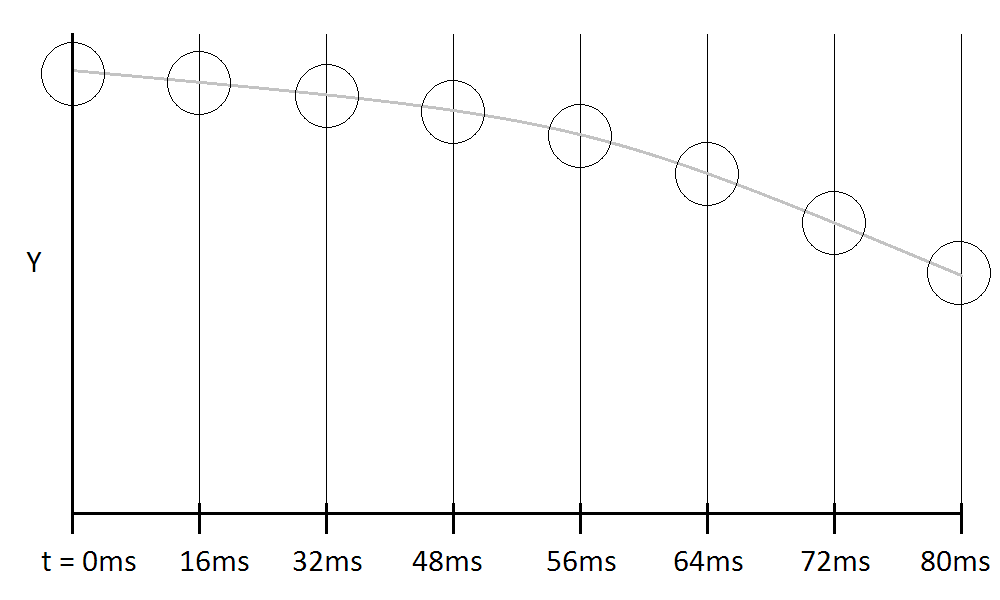
\includegraphics[width=6.0in]{images/TimeStepping}
	  \caption{Example of time stepping for a falling sphere. Time is split into discrete chunks, called \textit{frames},
	  and each frame advances the simulation by a \textit{time step} of 16 milliseconds(ms).}
	\end{figure}
	
	The update loop for such a particle system might be written as:
	\begin{itemize}
		\item Detect collisions
		\item Determine collision response forces
		\item Integrate velocity(that is, apply collision response forces and other forces such as gravity)
		\item Integrate position
	\end{itemize}
	
	Let's go over that loop in a bit more detail:
	\subparagraph{Detect collisions} 
	The main purpose of this stage is to generate information needed for the collision response stage. For each pair of 
	particles, we calculate a normal vector and distance. The normal vector, which is a vector of length 1 pointing from 
	one particle to another, determines the direction of the repulsive force used to separate the particles. The distance 
	determines whether a force needs to be applied and, if below 0 (which means that the particles are penetrating), 
	affects the magnitude of the force that is applied.
	\subparagraph{Determine collision response forces}
	In this stage, we generate forces that will change the velocities of the particles so that, ideally, they will not
	interpenetrate in the next step. The force is called the \textit{normal force} (as it is applied along the normal 
	vector), which scales up as large as needed to prevent the particles from penetrating. It is also possible to generate 
	a friction force, so that the particles will not slide across each other.
	
	\begin{figure}[ht]
	  \centering
	  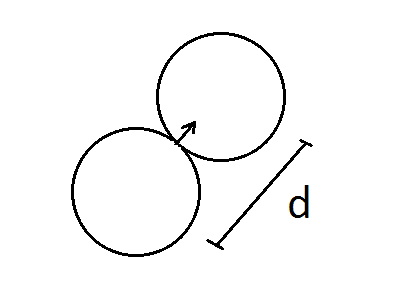
\includegraphics[width=3.0in]{images/SphereCollision}
	  \caption{The collision detection stage generates distance and a normal vector for each pair of colliding spheres.
	  If the spheres are able to rotate, then it is also necessary to detect the point of contact where the spheres are 
	  touching. Whether the normal vector points towards the left or right sphere is a matter of convention.}
	\end{figure}
	
	\subparagraph{Integrate velocity and position}
		In these stages, we advance the state of the simulation, updating the velocity and position of each particle.
		\[ \mathbf{velocity_{next} = velocity + (force/mass) * timestep} \]
		\[ \mathbf{position_{next} = position + velocity_{next} * timestep} \]
	It is important to note that we use \( velocity_{next} \) to compute the next position as opposed to the current 
	\(velocity\). This means that the velocity and position are integrated using semi-implicit Euler as opposed to
	explicit Euler. The difference is subtle but very important, as explicit Euler is unconditionally unstable;
	that is, it ensures that the simulation will explode if damping(artificially reducing the velocity) is not applied.\\
	
	\subsection{Extending the simple particle simulation to fluids}
	\subparagraph{\textit{Smoothed Particle Hydrodynamics}} may sound intimidating, but it is actually not very different from 
	this particle simulation. In particular, the only difference between a SPH fluid simulation and a rigid body particle 
	simulation is that the \textit{determine collision response forces} stage is different.\\
	
	To elaborate, the rigid body simulation uses a repulsive force between colliding particles, while an SPH fluid uses
	pressure and viscosity forces based on the \textit{Navier-Stokes equations}. This has the effect of changing some 
	characteristics of the particles. Instead of considering the particles as solid spheres of uniform density, with the
	mass evenly distributed across the particle, the particles are seen as points with a radius of interaction. 
	Furthermore, the boundary between SPH particles is soft. A common rule of thumb for SPH simulations is that each 
	particle should have 20--40 neighbors; that is, each particle is expected to be interpenetrating with 20 to 40 other
	particles. Finally, the mass of a SPH particle is unevenly distributed throughout the volume of the particle, with
	more mass concentrated at the center and less mass farther out.\\
	
	Another difference is that while rigid body particles are seen as distinct, separate entities, SPH particles are 
	viewed as being part of a fluid, with each SPH particle contributing to a greater whole. To be precise, each SPH 
	particle contributes some mass to a density scalar field. That is, it is possible to use particles to associate 
	every point in space with a density. Just as it is possible to use linear interpolation to define a line from 2 
	points, it is possible to use SPH to define a scalar field from many points.\\
	
	To reiterate, in addition to the properties of mass, radius, position, and velocity, SPH particles also gain the 
	implicit property of density. This property is not stored with each particle, but interpolated by summing the 
	contributions from all particles.\\
	
	\begin{figure}[ht]
	  \centering
	  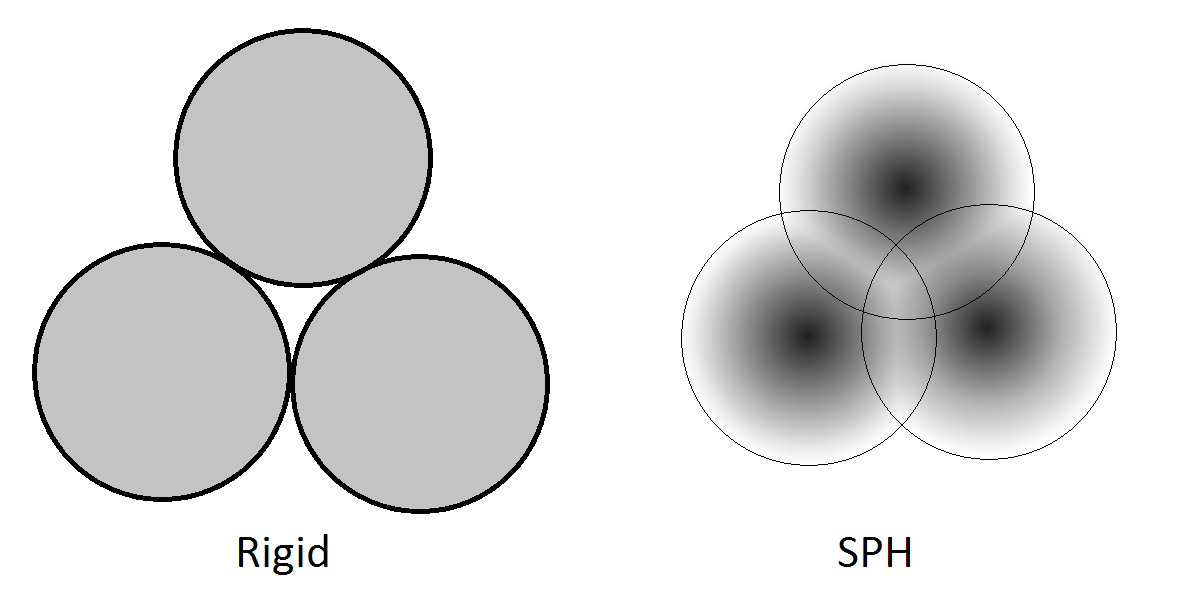
\includegraphics[width=6.0in]{images/RigidSPH}
	  \caption{On the left are uniform density rigid particles with hard boundaries. On the right are distributed density 
		SPH particles with soft boundaries. The darkness indicates the amount of mass at that point.}
	\end{figure}
	
	The equation we use to define the density, \(\rho\), at a position, \( \mathbf{r} \),  is:
	
	\begin{equation}
		\label{eq_density}
		\rho (\mathbf{r}) = \sum_{j}^{} m_j W_{poly6}(\mathbf{r} - \mathbf{r}_j, h)
	\end{equation}
	
	Where the sum loops over all nearby particles with position \( \mathbf{r}_j \) within the radius of interaction, 
	\( h \), the term \( m_j \) is the mass of a particle. \( W \) is used to denote a \textit{smoothing kernel}; it is
	a function that determines how a properity is distributed(or smoothed) throughout the volume of a fluid particle. 
	In this case, we are using the kernel named the \textit{poly6} kernel. In the context of our simulation, \( W_{poly6} \) 
	is a function that determines how the mass is distributed throughout a fluid particle. The amount of mass contributed is 
	highest at the particle's center, and gradually falls to 0 as the distance from the center increases to the radius of 
	interaction, \( h\).\\
	
	\begin{figure}[ht]
		\centering
		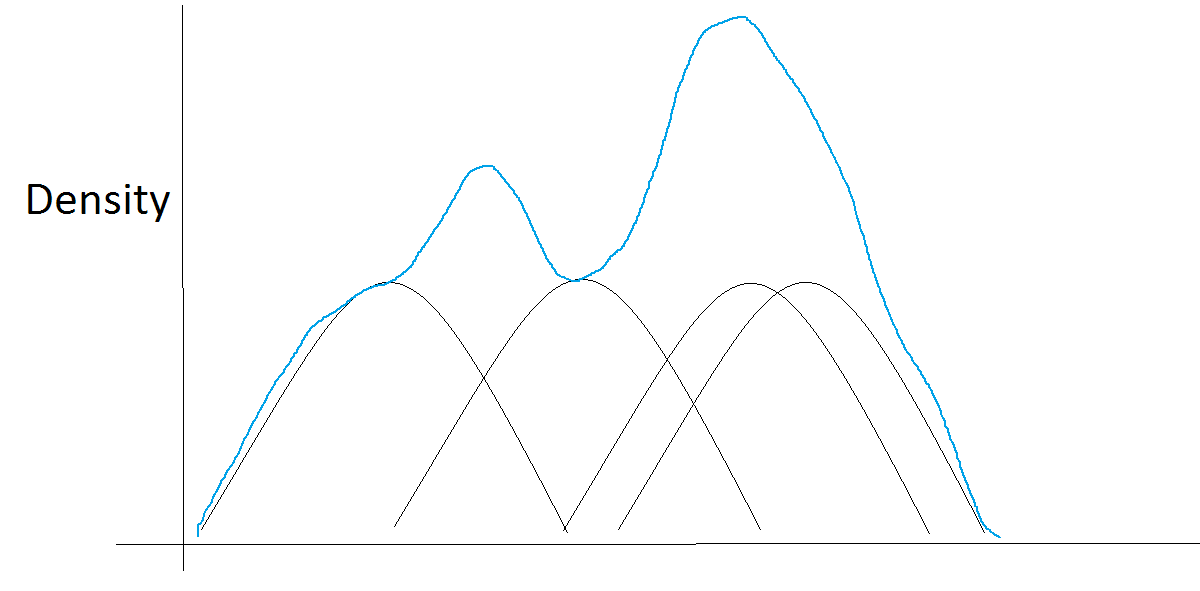
\includegraphics[width=6.0in]{images/SPHSum}
		\caption{Example of equation \ref{eq_density} in 1D. SPH Interpolates a global density(blue) by summing up local
		 densities(black) from particles.}
	\end{figure}
	
	Fluid motion is described by the the Navier-Stokes equations. Although the Navier-Stokes equations are a set of
	equations, we are only interested in a single equation due to various assumptions and other simplifications:
	
	\begin{equation}
		\rho \frac{\partial \mathbf{v}}{\partial t} = - \nabla p + \mu \nabla ^2 \mathbf{v} + \mathbf{f}
	\end{equation}

	With density \( \rho \), acceleration \( \partial \mathbf{v} / \partial t \), pressure \( p \), and velocity 
	\( \mathbf{v} \).
	
	This equation may appear complex, but it is actually quite simple; it is just \(F = ma\) for fluids.
	\begin{itemize}
		\item \(- \nabla p\), the negated gradient of pressure, means that fluids are accelerated from 
		places of higher pressure towards areas of lower pressure,
		\item \(\mu \nabla ^2 \mathbf{v}\), the Laplacian of velocity, means that fluid particles experience friction 
		against each other, with \(\mu\) being a constant that determines the amount of friction, and
		\item \(\mathbf{f}\) includes external forces such as gravity, surface tension and collision response forces
		 (for instance, forces from collisions with rigid bodies).
	\end{itemize}
	
	The main term in this equation that accounts for the motion of fluids such as water is the pressure term, 
	\(- \nabla p\). While the normal force that is applied between rigid body particles acts as a hard boundary that
	removes all penetration, the pressure force acts to eliminate variations in pressure. As we shall see next, 
	eliminating variations in pressure also has the effect of constraining the particles' density to a single value.\\
	
	Minor note: although the Laplacian operates on a scalar field, applying it to a vector simply means to apply it to
	each of the components and create another vector from the result. 
	\(\nabla ^2 \mathbf{v} = (\nabla ^2 v_x, \nabla ^2 v_y, \nabla ^2 v_z) \), where \(\mathbf{v} = (v_x, v_y, v_z)\).
	To be clear, there are 3 scalar fields(\(v_x\), \(v_y\), and \(v_z\)) involved in this expression.\\
	
	The density scalar field can be converted into a pressure field by using an equation of state. For liquids, the
	equation we use is:
	
	\begin{equation}
		\label{eq_densityToPressure}
		p = k(\rho - \rho_0)
	\end{equation}
	
	Where \( k \), the stiffness, is a positive constant that determines the strength of the pressure force and 
	\( \rho_0 \) is the fluid's rest density. The \textit{rest density} is exactly what it sounds like---the density of the 
	fluid when it is \textit{at rest}; that is, when it has settled and is not moving.\\
	
	The effect of this equation is that particles below \(\rho_0\), the rest density, will have a negative pressure, 
	while particles above the rest density will have a positive pressure. As the gradient operator points in the 
	direction of greatest increase, this results in a force that pushes the particles apart when above rest density,
	and together when below rest density.\\
	
	Now that we have a way of defining a pressure field, we have all the variables needed to approximate a solution
	for the acceleration using SPH. \(\mathbf{v}\) is carried by each particle and \(\rho\) can be calculated by 
	equation \ref{eq_density}.
	
	\begin{equation}
	acceleration = \frac{\partial \mathbf{v}}{\partial t} = \frac{- \nabla p + \mu \nabla ^2 \mathbf{v} + \mathbf{f}}{\rho}
	\end{equation}
	
	Using SPH, the term \(- \nabla p\) is approximated at a particle i as:
	
	\begin{equation}
		\mathbf{f}_{i}^{pressure} = - \sum_{j}^{} m_j \frac{p_i + p_j}{2 \rho_j} \nabla W_{spiky}(\mathbf{r}_i - \mathbf{r}_j, h)
	\end{equation}
	
	and the viscosity term \(\mu \nabla ^2 \mathbf{v} \) as:
	
	\begin{equation}
		\mathbf{f}_{i}^{viscosity} = \mu \sum_{j}^{} m_j \frac{ \mathbf{v}_j - \mathbf{v}_i}{\rho_j} \nabla ^ 2 W_{viscosity}(\mathbf{r}_i - \mathbf{r}_j, h)
	\end{equation}
	
	Where \( \nabla W_{spiky} \) is the gradient of the spiky kernel, and \( \nabla ^ 2 W_{viscosity} \) is the 
	Laplacian of the viscosity kernel. The spiky and viscosity kernels are functions that have been specially designed
	to improve stability when using SPH to approximate pressure and viscosity forces. Similiar to the \(W_{poly6}\) kernel,
	they scale the force between pairs of particles, with the force gradually dropping to 0 as the distance between particles
	increases to the radius of interaction.\\
	
	Substituting terms from the kernels \(W_{poly6}\), \(\nabla W_{spiky}\), and \(  \nabla ^ 2 W_{viscosity}\), 
	removing constant terms from the sum, and then solving for acceleration(\( \mathbf{f}_i = \rho_i \mathbf{a}_i \)) 
	changes the equations into this form:
	
	\begin{equation}
		\label{eq_densityFinal}
		\rho_i (\mathbf{r}_i) = \frac{315m}{64 \pi h^9 } \sum_{j}^{} (h^2 - (|\mathbf{r}_i - \mathbf{r}_j|)^2 )^3
	\end{equation}
	
	\begin{equation}
		\label{eq_pressureAccel}
		\mathbf{a}_{i}^{pressure} =  \frac{45 m}{\pi h^6}  \sum_{j}^{} \frac{p_i + p_j}{2 \rho_i \rho_j} 
		 \frac{\mathbf{r}_i - \mathbf{r}_j}{|\mathbf{r}_i - \mathbf{r}_j|} (h - |\mathbf{r}_i - \mathbf{r}_j|)^2 
	\end{equation}
	
	\begin{equation}
		\label{eq_viscosityAccel}
		\mathbf{a}_{i}^{viscosity} = \frac{45 \mu m}{\pi h^6} \sum_{j}^{} \frac{ \mathbf{v}_j - \mathbf{v}_i}{ \rho_i \rho_j} (h - |\mathbf{r}_i - \mathbf{r}_j|)
	\end{equation}
	
	Going over the terms again, \(m\) is the mass of a particle(assuming all particles have the same mass), \(h\) is the 
	radius of interaction, \(p\) is pressure, \(\rho\) is density, \(\mu\) is the strength of viscosity, \(\mathbf{r}\) 
	is position, and \(\mathbf{v}\) is velocity. The subscripts i and j are used to indicate the indices of the particles
	that the properties are associated with. \(|\mathbf{r}_i - \mathbf{r}_j|\) denotes the distance between points 
	\(\mathbf{r}_i\) and \(\mathbf{r}_j\). \\
	
	Every frame, we iterate over all particles twice. The first pass to calculate the density and pressure (equations 
	\ref{eq_densityFinal} and \ref{eq_densityToPressure}), and the second pass to calculate pressure and viscosity forces
	(equations \ref{eq_pressureAccel} and \ref{eq_viscosityAccel}). Finally, we apply these forces to each particle, 
	and integrate their positions.\\
	
	To conclude, there is only a minor conceptual difference between a rigid body particle simulation and a SPH fluid 
	simulation. In order to convert a rigid body particle simulation into a SPH fluid simulation, we need only to 
	replace the repulsive force with pressure and viscosity forces.\\
	
	The important things to remember are that: 
	\begin{itemize}
		\item Fluid motion is described by the Navier-Stokes equations, which define a pressure and viscosity force.
		\item SPH is a method that combines the local contributions of particles to represent a global scalar field, 
		and can be used to approximate solutions to the Navier-Stokes equations.
		\item The SPH pressure force is both attractive and repulsive, and accelerates particles towards the fluid's 
		rest density.
		\item The SPH viscosity force accelerates particles towards having the same velocity. This has a similar effect
		to friction, dissipating energy and gradually reducing the velocity of the particles. (2 particles with the 
		same velocity experience no acceleration from the viscosity force, while particles moving in opposite directions 
		experience a strong viscosity force.)
	\end{itemize}
	
	The derivation presented in this article was originally introduced by M\"{u}ller, Charypar, and Gross in 
	\cite{Muller:2003:PFS:846276.846298}. It is recommended to see their paper for a more in depth explanation. 
	Additionally, a good tutorial on SPH is provided in Kelager's Master's thesis \cite{MK:2006}.\\
	
	For completeness, the definitions of the kernels are presented here:\\
	
	Poly6 kernel:
	\begin{equation}
		W_{poly6}(\mathbf{r} - \mathbf{r}_j, h) = 
			\left \{ 
				\begin{array}{ll}
					\dfrac{315}{64 \pi h^9 } (h^2 - (|\mathbf{r} - \mathbf{r}_j|)^2)^3 
						& \textrm{if \(0 \leq |\mathbf{r} - \mathbf{r}_j| \leq h\) } \\[1em]
					0 & \textrm{otherwise} 
				\end{array}
			\right.
	\end{equation}
	
	Gradient of spiky kernel:
	\begin{equation}
		\nabla W_{spiky}(\mathbf{r} - \mathbf{r}_j, h) =  
				\left \{ 
					\begin{array}{ll}
						- \dfrac{45}{\pi h^6}  \dfrac{\mathbf{r} - \mathbf{r}_j}{|\mathbf{r} - \mathbf{r}_j|} 
							(h - |\mathbf{r} - \mathbf{r}_j|)^2 
							& \textrm{if \(0 \leq |\mathbf{r} - \mathbf{r}_j| \leq h\) } \\[1em]
						0 & \textrm{otherwise} 
					\end{array}
				\right.
	\end{equation}
	
	Laplacian of viscosity kernel:
	\begin{equation}
		\nabla ^ 2 W_{viscosity}(\mathbf{r} - \mathbf{r}_j, h) =  
						\left \{ 
							\begin{array}{ll}
								\dfrac{45}{\pi h^6} (h - |\mathbf{r} - \mathbf{r}_j|)
									& \textrm{if \(0 \leq |\mathbf{r} - \mathbf{r}_j| \leq h\) } \\[1em]
								0 & \textrm{otherwise} 
							\end{array}
						\right.
	\end{equation}
	
\pagebreak
\section{Parameters}
	In the context of real time simulations, factors such as the time step and low stiffness mean that the relation to
	physical units becomes largely academic, so using actual physical values is unlikely to give the desired result. 
	Parameters at world scale are marked as [world scale] and parameters at simulation scale are marked as 
	[simulation scale]. [X, Y] means that the range of the parameter should be between X and Y. For instance, [0.0, 1.0]
	denotes a range from 0 to 1.
	
	\subsection{Global Parameters}
		Properities assigned to all btFluidSph in a btFluidRigidDynamicsWorld.
	
		\subparagraph{m\_timeStep}
			For performance and stability reasons, it is not possible to run the fluid simulation at the same time step as 
			the rigid body simulation. Setting this value too high will cause the fluid to explode. In general, a higher 
			time step requires lower stiffness to prevent the fluid from exploding. As a rule of thumb, doubling the time step
			means that the stiffness needs to be halved. By default, the fluid is stepped 5 times slower(3ms) than the rigid body simulation(16ms).
		
		\subparagraph{m\_simulationScale}
			See \ref{s_simulationScale}.
		
		\subparagraph{m\_gravity [simulation scale] }
			Acceleration applied to all particles during each frame; by default the Y- axis is assumed to point downwards.
			Note that, as this is a simulation scale parameter, the default gravity is 250x larger compared to rigid bodies. 
			This default value can be reduced considerably. (Part of the reason for the high default gravity is the ratio of 
			time steps between fluid/rigid).
		
		\subparagraph{m\_sphSmoothRadius [simulation scale]}
			Commonly denoted as \(r\) or \(h\) in the literature. Defines the radius in which SPH particles will 
			interact with each other. This should be set so that each particle has about 20--40 neighbors. To be precise, 
			a particle influences another if the distance to its center is less than or equal to \(r\)---that is, it 
			should be thought of as sphere v. point collision. Considering it as sphere-sphere collision means that both
			spheres would have a radius of \(r/2\).
		
	\subsection{Local Parameters}
		Properties assigned to a single btFluidSph.

		\subsubsection{Fluid Simulation}
			\subparagraph{m\_viscosity}
				Affects the magnitude of the viscosity force, which accelerates particles so that they have the
				same velocity---it defines the resistance of the fluid to flow. For instance, water has low viscosity while 
				honey has high viscosity. The viscosity force also works to improve the numerical stability of the simulation
				by reducing particle velocities(setting this to 0 can cause the fluid to explode). However, a too high viscosity 
				value will instead introduce energy into the simulation.\\
				
				This is the parameter \(\mu\) in equation \ref{eq_viscosityAccel}.
			
			\subparagraph{m\_restDensity}
				Defines the density of the fluid when it is at rest, or not moving. Water has a rest density
				of \(1000 kg / m^3\). The pressure force is applied to constrain particles to this density.
				
			\subparagraph{m\_sphParticleMass}
				Contribution of a single particle to the SPH density scalar field.
				
			\subparagraph{m\_stiffness [simulation scale]}
				The fluid stiffness determines how violently the fluid reacts to variations in density. In other words, it
				defines the magnitude of the SPH pressure force. For mostly incompressible fluids such as water, is best to
				keep this value as high as possible. Another reason to use a higher stiffness value is performance; a particle
				that is part of a compressible(low stiffness) fluid tends to have more neighbor particles. The maximum stiffness
				that can be used is dependent on the time step.\\
				
				This is the parameter \(k\) in equation \ref{eq_densityToPressure}.
			
			\subparagraph{m\_initialSum (0.0, 1.0]}
				Determines the particle's self contribution when calculating its density. It should always be greater than 0,
				but generally be kept as low as possible. Using a value of 1 is equivalent to adding a virtual SPH particle at zero distance
				when calculating each particle's density; the virtual particle is not included when calculating forces.
				
				Higher values improve stability, especially for particles that are isolated or have incomplete neighborhoods. 
				As it has the effect of increasing the density of all particles, however, it also tends to make particles repulse
				each other more strongly.
				
			\subparagraph{m\_particleDist [simulation scale]}
				This is an automatically calculated value that defines a default spacing for particles. It has no effect on
				the simulation, but should not be changed. Consider spawning a group of fluid particles in the shape of a 
				box. Placing the fluid particles too far apart will cause them to attract(box implodes), while spacing them
				too closely will make them repulse(box explodes). Depending on how m\_initialSum is set, this may need to
				be scaled by a factor of 0.75--1.25.
		
		\subsubsection{Rigid Body Interaction}
			\subparagraph{m\_particleRadius [world scale]}
				Radius of a particle with colliding with btRigidBodies/btCollisionObjects. The particle is treated as a rigid body sphere.
				Has no effect on the SPH simulation. Note that this is separate from m\_sphSmoothRadius, which defines the radius for
				interactions between fluid particles.
				
			\subparagraph{m\_particleMargin [0.0, m\_particleRadius) [world scale]}
				Meters of allowed penetration when colliding with rigid bodies. This value should be a small fraction of
				m\_particleRadius. Should not be set to 0, as it can cause fluid particles to oscillate when colliding
				with rigid bodies(also known as jitter).
				
			\subparagraph{m\_particleMass}
				Mass of a particle when interacting with rigid bodies and applying forces.
				
			\subparagraph{m\_particleRadiusExpansion [world scale]}
				Expands the collision detection radius of a particle. Can be used to find objects that are near but not
				colliding with the fluid particles. Setting this too high will reduce performance and degrade the accuracy
				of fluid-rigid contacts.
				
			\subparagraph{m\_boundaryFriction [0.0, 1.0]}
				Fraction of tangential velocity to remove per frame when a fluid particle collides with a rigid body. For 
				example, using a m\_boundaryFriction of 0.2 would cause a tangential velocity with magnitude 1 to be 
				reduced to 0.8 after 1 frame. In practice, a value of e.g. 0.2 is already very high. Setting this too high 
				will cause instablility.
				
			\subparagraph{m\_boundaryRestitution [0.0, 1.0]}
				Generally set to 0 for fluids. It controls the fraction of normal velocity that is reflected when a fluid 
				particle collides. Using a nonzero value will cause particles to bounce off rigid bodies when colliding. 
				Note this introduces energy into the system, so it will make the fluid less stable.
				
			\subparagraph{m\_boundaryErp [0.0, 1.0]}
				The boundary ERP(Error Reduction Parameter) controls the fraction of penetration removed per frame from
			fluid-rigid contacts. Higher values reduce penetration more quickly, but at the cost of lower stability.
		
	\subsection{Other Parameters}
		\subparagraph{setCcdMotionThreshold}
			The function btCollisionObject::setCcdMotionThreshold(), inherited by btFluidSph,
			can be used to prevent fluid particles from tunneling through rigid bodies.
			There is no feature to prevent rigid bodies from tunneling through fluids.
			In general, this should be set to btFluidSphParametersLocal.m\_particleRadius.
			
\pagebreak		
\section{Optimizations}
	Implementing a basic SPH algorithm is actually quite simple. Without any optimizations, 
	it would simply take the form of a double nested loop. Much of the complexity comes from the grid algorithm.
		
	\subsection{Grid Algorithm}
		For spheres of the same radius, the most efficient algorithm is a uniform grid.
		That is, we divide space into unformly sized cubes(or cells) that are axis-aligned. 
		We add particles into these cells by checking which cell the particle's center is in. 
		If the edge length of the cells is equal to the SPH interaction radius, then the particles
		that are able to interact with a particle are in the directly adjacent cells.
		
		There are several ways of implementing the uniform grid, some are presented here.\\
		
		\subsubsection{Static Noncolliding Uniform Grid (implemented by Bullet-Fluids) }
			It is a fixed-size sparse implicit grid, where only the contents of grid cells containing particles is stored.
			
			The main advantage of this grid is that it has no collisions, and can be used in a fairly large world. 
			The main disadvantage is that it requires a binary search to query a cell.\\
			
			The information maintained by this algorithm includes:
			\begin{itemize}
				\item Cell size: A scalar. This is identical to the SPH interaction radius.
				\item value[]: An array containing \textit{hash values} that identify grid cells. Each value is a 32-bit or 
				64-bit int. 10 or 21 bits are used for each dimension(x, y, z), so that worlds of \(1024^3\) and 
				\(2097152^3\) cells can be used.
				\item index\_range[]: An array containing the range of particle indicies that correspondes to each grid
				cell. Each element containts 2 32-bit ints that store the first and last index of the particles in each
				grid cell.
				\item value\_index[]: An array containing value-index pairs. Where the index identifies a particle and the
				\textit{value} identifies the grid cell it is inside. There is one entry in this array for each particle.
			\end{itemize}
			
			value[] and index\_range[] are parallel arrays, so value[i] identifies the grid cell with index i and contents 
			index\_range[i]. The length of the value[] and index\_range[] array is equal to the number of grid cells with 
			particles in them.\\
			
			Grid Update Algorithm:
			\begin{enumerate}
				\item Quantize\\
				First, a particle's position is converted into integer grid cell coordinates( \( \mathbb{R}^{3} \to \mathbb{Z}^{3}\) ).
				This is achieved by dividing each coordinate of the particle's position by the grid cell width.
				Since a simple division would result in the cell (0,0,0) having a size of \(2r\), we map the coordinate 
				in range [0, r) to 0, and [-r, 0) to -1. Converts the continuous coordinates \((x, y, z)\) to the integer 
				coordinates \((x_{grid}, y_{grid}, z_{grid})\).
				
				\item Assign value with hash function\\
				Next, we combine these coordinates into a single value that can be used for sorting.
				\begin{equation}
					\label{eq_hash}
				value = x_{grid} + y_{grid} * C + z_{grid} * C * C
				\end{equation}
				where C = 1024 or 2097152, defines the maximum extent of the grid in each dimension.
				
				\item Create value-index pairs\\
				We associate each particle with its value for sorting, creating an array of structs, each struct a 
				{value, index} pair.
				
				\item Sort by value-index pairs by value\\
				On CPU, quick sort is used while radix sort is used on GPU. After sorting the particles are grouped by 
				grid cells. The result of this step is an array of value-index pairs, where value\_index[i] is the current 
				position and value\_index[i].index is the last position.
			
				\item Rearrange particles\\
				In order to avoid consuming a large amount of memory bandwidth during the sort, we only sort value-index 
				pairs and then rearrange other particle attributes (position, velocity, user-pointer, etc.) after the sort.
			
				\item Generate index ranges\\
				Look through the particles to get the range of particle indicies corresponding to each grid cell.
				
				The result of this stage is a set of [value, index-ranges] pairs; the value is used to identify
				the grid cell, and the index-range indicates its contents.
			\end{enumerate}
			
			Grid Query Algorithm:
			\begin{enumerate}
				\item Quantize
				\item Assign value\\
				In order to find neighbors, the first 2 steps is the same as the grid update.
				\item Binary Search\\
				Perform a binary search for the cell with value, once we have the index of the cell, it
				can be used to access the particle index range. Although a binary search may sound expensive, 
				it only needs to be performed for each grid cell.
			\end{enumerate}
			
		%\subsubsection{Modulo Colliding Uniform Grid}
		%	By using the hash function X % C + (Y % C) * C + (Z % C) * C * C, a finite grid can be extended into an infinite domain.\\
		%	(e.g. C = 64)
		%
		%	A drawback of this method is collisions. Another is that the '3-cell bar' optimization cannot be used without 
		%	adding an additional branch to distinguish between outer and inner cells.\\
		%	
		%	More information on this grid may be found in:
		%	NVIDIA particles presentation[REFERENCE]
		%	PhysX presentation reference[REFERENCE]
			
	\subsection{Grid Cell Size}
		The cell size \(r * (3^3)\) is the optimal size for a CPU/GPU implementation.
		Compared to \(2r * (2^3)\), it contains half the volume, so it is a closer fit to the actual neighbors.
		
		On CPU, it also simplifies the symmetry optimization; since each particle in the same cell has the same
		26 neighbor cells, it becomes possible to do processing on each grid cell instead of each particle.
		(It is actually possible to use the symmetry optimization with 2r cells, but it is much more complicated.
		The method requires making a copy of the grid and removing particles from the cell as the SPH density 
		and SPH force is calculated. Additionally, since each 2r grid cell can still access 26 neighbors overall,
		it is still necessary to split the cells into 27 groups for multithreading, which reduces the amount of
		parallelism as each 2r cell has 8 times the volume of a r cell)
	
	\subsection{GPU Optimizations}
		On the GPU, we found that it is more efficient to store density and recompute the pressure instead of storing 
		the inverted density and pressure. Using the ternary operator and moving the (i != n) to the distance check also 
		helps reduce divergence.\\
		
		\subsubsection{3-cell bar}
			If the hash function is defined as in the Bullet-Fluids grid(equation \ref{eq_hash}), it becomes possible
			to group 3 cells into a 3-cell bar, which reduces the amount of divergence. Instead of processing
			27 cells, 9 3-cell bars are processed.
			
			\begin{figure}[ht]
			  \centering
				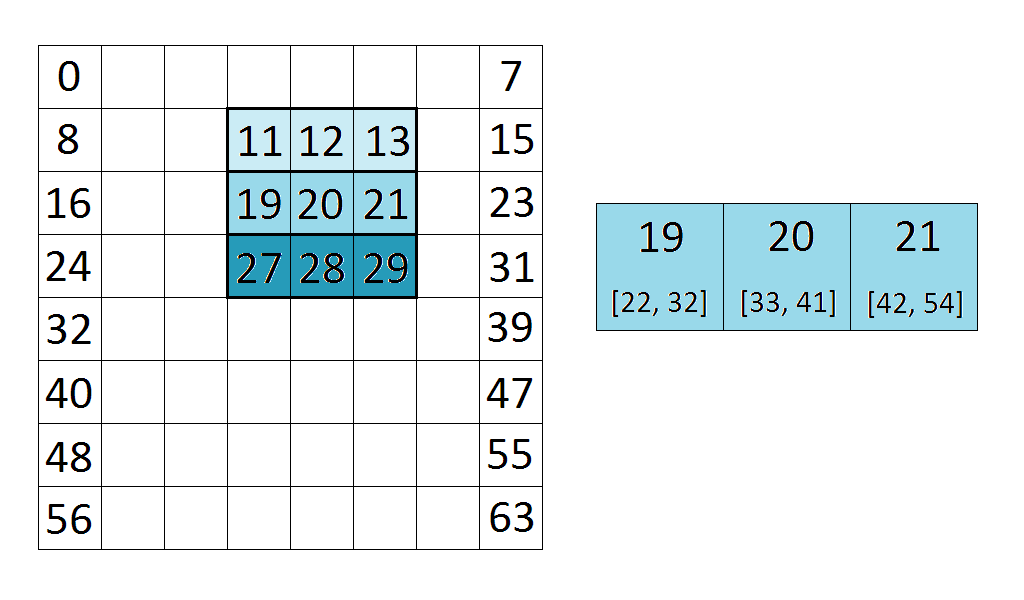
\includegraphics[width=6.0in]{images/3CellBar}
				\caption{2D example of 3-cell bar optimization. In this case, the constant C in equation \ref{eq_hash} is 
				equal to 8. Instead of using a for loop with 9 iterations(27 in 3D), it is possible to use a for loop with 3
				iterations(9 in 3D), with each iteration processing 3 cells. In this example, the cells with values 19, 20, 
				and 21 have particles with indicies [22, 32], [33, 41], and [42, 54], respectively. Instead of running 3 
				iterations for each of these particle index ranges, we can perform a single iteration through the range [22, 54].}
			\end{figure}
		
		\subsubsection{Effect of CPU optimizations on the GPU}
			\subparagraph{Neighbor table}
				Although using neighbor tables improves performance on CPU, it decreases overall performance and 
				increases memory consumption on the GPU. To be exact, it reduces the performance of the density
				computation stage and improves the performance of the force calculations stage. There may be a 
				performance benefit for methods that iterate over all particles several times, however.
			\subparagraph{Symmetry}
				Implementing the symmetry optimization as on CPU was found to result in a \(\sim\)50x performance decrease.
				This is likely because:
				\begin{itemize}
					\item Processing by grid cell requires more registers.
					\item Higher memory latency on GPU means that the symmetric optimization is less effective.
					\item There are less grid cells than particles, which reduces the max number of active threads.
					Additionally, grouping the cells into 27 groups further reduces the occupancy. A GPU typically needs
					1000--10000 or more threads for efficient processing. On average, a grid cell with size \(r\) has 4
					particles and 27 groups are needed to avoid thread collisions, so the overall number of threads that
					can be used is reduced by an estimate of \(4 * 27 = 108\).
				\end{itemize}
			
	\subsection{CPU Optimizations}
		\subsubsection{Symmetry and Multithreading}
			In order to allow multithreading without using atomics or other syncronization, the grid cells are divided 
			into 27 groups (9 groups in 2D) so that processing all the cells in a single group will not cause thread 
			collisions.
			
			Since the pressure and viscosity forces are antisymmetric, that is, \(\mathbf{f}_{ij} = - \mathbf{f}_{ji}\),
			it is only necessary to compute forces once for each pair of particles. The density contribution between 
			particles is also symmetric, so the same optimization can be applied during the density computation stage. 
			This additionally reduces the number of neighbor cells that needs to be accessed by each cell from 26 to 
			13 cells in 3D and 8 to 4 cells in 2D.
			
			\begin{figure}[ht]
			  \centering
				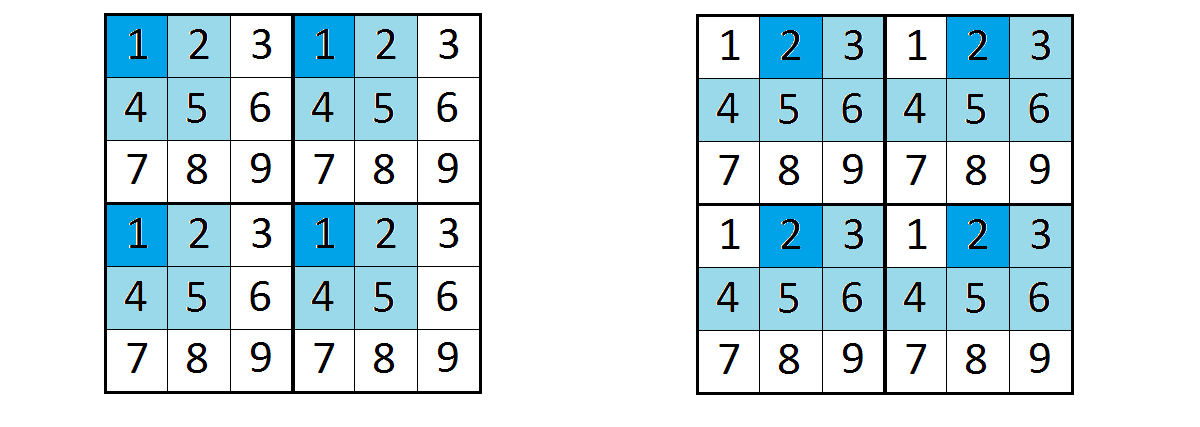
\includegraphics[width=6.0in]{images/CellGrouping}
				\caption{Multithreading optimization. A 2D example is presented for 2 iterations. The cells are grouped
				into clusters of 9 cells, and due to symmetry each cell only needs to access 4 neighbor cells during 
				the computation. During the first iteration, cells marked 1 can be processed by multiple threads. During
				the second iteration, cells marked 2 are processed, and so on. Dark blue indicates the current cell,
				while light blue indicates neighbor cells that are accessed and written to. }
			\end{figure}
		\subsubsection{Neighbor Tables}
			The index and distance of neighbor particles are stored during the SPH density calculation to avoid
			recomputing during the SPH force calculation. Due to symmetry, each entry represents a pair.
			This also allows tuning the quality of the simulation by reducing the max number of neighbors.

\pagebreak			
\section{Other Internal Details}
	\subsection{Update Loop}
		\begin{enumerate}
			\item Update grid
			\item Calculate SPH sum (density and pressure)
			\item Calculate SPH pressure and viscosity force
			\item Integrate velocity (apply SPH forces)
			\item Handle collision detection and response with rigid bodies (correct velocities to avoid penetrating into rigids)
			\item Integrate position
		\end{enumerate}
	
	\subsection{Rigid Body Interaction}
		Fluid-Rigid interaction is implemented by treating particles as rigid body spheres.
		CCD is implemented for moving fluid against rigid by casting a ray along the path of
		a fluid particle's motion. If the ray intersects a rigid body, then the particle is moved
		to intersect slightly with the rigid body. The collision response step then prevents the particle
		from tunneling by applying an impulse that is as large as needed.\\
		
		To describe the collision resolution method, the force has 2 components. The first force(or \textit{impulsive force}) 
		prevents the particle from further penetrating, by scaling as large as needed to remove the component of the velocity
		in the direction of penetration. The second force, scaled by m\_boundaryErp, removes penetration.\\
		
		A drawback of this method is that fluid particles can stack while colliding with rigid bodies.
		That is, since the fluid is not completely incompressible, many fluid particles can occupy the same
		space and, as a result, cause a collding rigid body to experience very strong collision forces. This issue is
		reduced somewhat if a less compressible, but more expensive, fluid simulation method is used.\\
		
		Another limitation is that the SPH density is inaccurate at boundaries, as SPH assumes that
		each particle has a full neighborhood. This causes fluids to cluster at boundaries in order to make 
		up for the reduction in density.\\
		
		Dynamic rigid bodies, especially triangle meshes, are able to tunnel through the fluid
		if moving too fast. Currently, there is no solution for this issue aside from reducing the
		time step.
	
	\subsection{Other notes}		
		\subparagraph{Clustering}
			When implementing a new SPH solver, a common issue is that the particles only seem to attract each other 
			and form into clumps. This may be caused by using the incorrect sign for the pressure force(or a negative 
			stiffness).
		\subparagraph{Split masses}
			The mass of a particle is different when calculating the SPH force and when interacting with rigid bodies.
			This allows the user to separately tune the interaction with rigid bodies. Another motivation is that large
			mass ratios between rigid bodies can cause the simulation to become unstable.
		\subparagraph{Local and Global parameters split}
			In order to efficiently perform fluid-fluid interaction, it is necessary to use a common smoothing radius 
			and simulation scale. Otherwise, the grids would be out of alignment and a more complex approach that is 
			also slower would be needed.
		\subparagraph{Denormalized floating point}
			The variables used by SPH can become very close to 0, causing the floating point values to become 
			denormalized. This has the potential to cause extreme degradations in performance, although the author has 
			not encountered such issues even with 32-bit floats.

%\pagebreak
%\section{Recommended Reading}
%	\subsection{Grid Algorithm}
%	\subsection{Incompressibility}
%	\subsection{Rendering}

\pagebreak
\bibliographystyle{plain}
\bibliography{BulletFluids_reference}		
\end{document}
